\section{Elkies' Small Values}\label{sec:targets}

Elkies~\cite{Elkies1996} found fractions, ups and tinies in chess endgames on the ordinary board. We searched
the census (Section~\ref{sec:atlas}) for smaller values of these kinds: $1/8$, $1/16$ and $1/32$;
\emph{up-second} $\upsec=\game{0}{{\downarrow}\star}$, positive but smaller than ${\uparrow}$, and
$\upsec\star=\game{0,\star}{{\downarrow}}$; and the \emph{tinies} $\tinyg{x}=\ggame{0}{0\mid -x}$ (a number $x$).
Table~\ref{tab:targets} counts them under both passed-pawn tests; under the e.p.-aware test $1/32$
disappears.

\begin{table}[!t]
\caption{Elkies' Small Values in the Census}
\label{tab:targets}
\centering
\begin{tabular}{@{}llcc@{}}
\toprule
Value & Form & Textbook & E.p.-aware \\
\midrule
$1/8$ & $\game{0}{1/4}$ & $13$ & $9$ \\
$1/16$ & $\game{0}{1/8}$ & $3$ & $2$ \\
$1/32$ & $\game{0}{1/16}$ & $1$ & $0$ \\
$\upsec$ & $\game{0}{{\downarrow}\star}$ & $5$ & $2$ \\
$\upsec\star$ & $\game{0,\star}{{\downarrow}}$ & $10$ & $10$ \\
$\tinyg{1}$ & $\ggame{0}{0\mid -1}$ & $13$ & $16$ \\
$\tinyg{x}$, $x\notin\mathbb{Z}$ & $\ggame{0}{0\mid -x}$ & $0$ & $0$ \\
\bottomrule
\end{tabular}

\smallskip
\parbox{\columnwidth}{\footnotesize Positions of each exact value in the census (count rule). Textbook
column: an independent C solver confirmed each identity (position minus target $=0$) \lab{C2}. E.p.-aware
column: \lab{C1}.}
\end{table}

\begin{figure}[!t]
\centering
\begin{subfigure}[b]{0.32\columnwidth}\centering
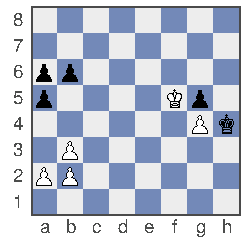
\includegraphics[width=\linewidth]{figures/eighth.pdf}
\caption{}
\end{subfigure}\hfill
\begin{subfigure}[b]{0.32\columnwidth}\centering
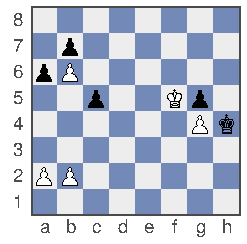
\includegraphics[width=\linewidth]{figures/upsecstar.pdf}
\caption{}
\end{subfigure}\hfill
\begin{subfigure}[b]{0.32\columnwidth}\centering
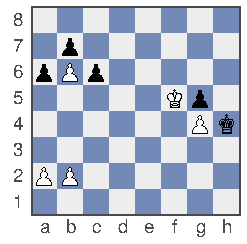
\includegraphics[width=\linewidth]{figures/tiny1.pdf}
\caption{}
\end{subfigure}
\caption{Elkies' small values beside T (Fig.~\ref{fig:trebuchet}), each a 10-man position with a legal pawn
history (ordinary board). (a)~$1/8$: \pos{W a2 b2 b3 / B a5 a6 b6}. (b)~$\upsec\star$: \pos{W a2 b2 b6 / B a6 b7 c5}.
(c)~$\tinyg{1}$: \pos{W a2 b2 b6 / B a6 b7 c6}.}
\label{fig:eighth}
\end{figure}

\subsection{A Reachable Eighth}

\begin{theorem}[\lab{C2}]\label{thm:eighth}
In the pawn model, white a2, b2, b3 against black a5, a6, b6 has value exactly $1/8$ in all nine settings
(Section~\ref{sec:ep}) and for every assignment of outcomes to its race positions.
\end{theorem}

To see why, look at Fig.~\ref{fig:eighth}(a). If white moves first, a2--a4 locks the a-file and leaves the
zero game. The quieter a2--a3 reaches only $\star$, from which black can return to $0$, so it is reversible.
The move b3--b4 is bad, since black's reply leaves $-3$. If black moves first, b6--b5 leaves $1/4$, and
a5--a4 is bad. Thus $G=\game{0}{1/4}=1/8$.

This pawn structure can arise in a game: from the starting position, c2$\times$b3, a7--a5, b7$\times$a6 and
c7$\times$b6 produce it. Its mirror image, white a2, a3, b2 against black a6, b5, b6, cannot, since its
a3-pawn could only have come from a2 or b2, and both are still on their starting squares. The independent
checks were run on the mirror, which has the same value by symmetry: a C solver confirms both parts of the
theorem, and a third, separately written solver confirms the value in all nine settings. Section~\ref{sec:real} tests the $1/8$ with real kings.

\subsection{Up-Second Star and Tiny~1}
White a2, b2, b6 against black a6, b7, c5 (Fig.~\ref{fig:eighth}(b)) is $\upsec\star$ in all nine settings
\lab{C2}. If white moves first, a2--a4 leaves $0$ and a2--a3 leaves $\star$. If black moves first, a6--a5
leaves ${\downarrow}$. Thus $G=\game{0,\star}{{\downarrow}}=\upsec\star$.

Now move the black c-pawn back to c6 (Fig.~\ref{fig:eighth}(c)). If white moves first, a2--a3 leaves $0$.
If black moves first, a6--a5 leaves $-1/2\pm1/2=\game{0}{-1}$, and c6--c5, which reaches the $\upsec\star$
position, is dominated, since $\game{0}{-1}\le\upsec\star$. Thus $G=\ggame{0}{0\mid -1}=\tinyg{1}$ under
every race rule with en passant on (textbook test \lab{C2}, e.p.-aware test \lab{C1}); with e.p.\ off it is
${\uparrow}$. Unlike the Tiny~1 of Section~\ref{sec:basic-inf}, it needs no seam. Both pawn structures
arise from the starting position by c2$\times$b3, b3--b4--b5--b6, a7--a6 and c7--c5 (c7--c6 for Tiny~1).

\subsection{Two Textbook Values That Fail}
Under the textbook test the census also has a $1/8$ at white a2, b2, d2 against black a5, c4, d7 and an
$\upsec$ at white a3, c5, d4 against black a7, b7, d7. The e.p.-aware test makes them $-3/2\pm3/2$ and
$\game{3/4}{{\downarrow}\star}$. Both rested on counting as passed a pawn that
could still be taken en passant. This is why we state Theorem~\ref{thm:eighth} and the $\upsec\star$ above for
all nine settings.
